% This is samplepaper.tex, a sample chapter demonstrating the
% LLNCS macro package for Springer Computer Science proceedings;
% Version 2.20 of 2017/10/04
%
\documentclass[runningheads]{llncs}
%
\usepackage{amsmath}
\usepackage{graphicx}
\usepackage[toc,page]{appendix}
\usepackage{listings}
\usepackage{color}
\lstset{
  basicstyle=\ttfamily,
  columns=fullflexible,
%  frame=single,
  breaklines=true,
}

% Used for displaying a sample figure. If possible, figure files should
% be included in EPS format.
%
% If you use the hyperref package, please uncomment the following line
% to display URLs in blue roman font according to Springer's eBook style:
% \renewcommand\UrlFont{\color{blue}\rmfamily}

\begin{document}
%
\title{Reinforcement learning - Lab 3}
%
%\titlerunning{Abbreviated paper title}
% If the paper title is too long for the running head, you can set
% an abbreviated paper title here
%
\author{Dimitri Diomaiuta - 30598109}
%
% \authorrunning{F. Author et al.}
% First names are abbreviated in the running head.
% If there are more than two authors, 'et al.' is used.
%
\institute{University of Southampton}
%% \institute{Princeton University, Princeton NJ 08544, USA \and
%% Springer Heidelberg, Tiergartenstr. 17, 69121 Heidelberg, Germany
%% \email{lncs@springer.com}\\
%% \url{http://www.springer.com/gp/computer-science/lncs} \and
%% ABC Institute, Rupert-Karls-University Heidelberg, Heidelberg, Germany\\
%% \email{\{abc,lncs\}@uni-heidelberg.de}}
%
\maketitle              % typeset the header of the contribution
%
%% \begin{abstract}
%% Searching is one of the oldest artificial intelligence techniques used for problem solving. In this paper we analyze the results and scalability of both uninformed and informed search algorithms.
%% %\keywords{First keyword  \and Second keyword \and Another keyword.}
%% \end{abstract}
%
%
%

\section{Answer 1}
In a 2-player capture the flag game with 2 flags, 5 sites and 100
rounds we have a frequency distribution, which describes how many
times a site has been selected. The hider claims that the distribution
shown by equation \ref{hdist} is correct.
\begin{equation}\label{hdist}
H_{dist} = (47, 53, 31, 36, 34)
\end{equation}
The seeker claims, correctly, that this distribution is
incorrect. Since the hider selects 2 sites at each timestep $t$ the
sum of the frequency distribution should be consistent with equation
\ref{cons}, where $T$ is the number of rounds and $dist$ a frequency distribution.
\begin{equation}\label{cons}
  \sum_{i = 1}^{|dist|}x_i = flags * T
\end{equation}
Equation \ref{cons} does not hold for the hider distribution, in fact,
we have a total sum of $201$ ($\sum_{x_i \in H_{dist}}^{sites}x_i$)
which is bigger than $200$ ($flags * T$). The frequency distribution
described by equation \ref{newdist} respects the constraint described
by equation \ref{cons} and, hence, can be a correct frequency
distribution for the outlined game setting.
\begin{equation}\label{newdist}
  H_{newdist} = (102, 26, 24, 40, 8)
\end{equation}

\section{Answer 2}
Given the hider's frequency distribution described by equation \ref{hdist2}
we want to derive the best fixed guess strategy for the seeker.
\begin{equation}\label{hdist2}
  H_{dist} = (36, 24, 40, 63, 37)
\end{equation}
A fixed guessed strategy is a type of strategy that does not change
over time and that involves selecting the same action at each
timestep (the same two sites in a capture the flag game setting). In a
capture the flag game setting with 2 flags a fixed strategy is any
binary combination of the sites where the flags can be hidden. Given
distribution described by equation \ref{hdist2}, the best fixed
strategy for the seeker is to take the action described by equation
\ref{besta}.
\begin{equation}\label{besta}
  a_{best} = <x_3, x_4> where \:x_3, x_4 \in H_{dist}
\end{equation}
In equation \ref{besta}, $x_3$ and $x_4$ describe the sites where the
hider puts the flags more often, respectively $40$ and $63$ times. The
best fixed strategy for the seeker, hence, is to select the two sites
where the flags are most frequently hidden.

\section{Answer 3}
In this section we describe the implementation of different online
learning algorithms to play the capture the flag game. Capture the
flag is a game with a nonassociative setting, meaning that an agent
has to learn which action to take in just one situation that repeats
for $T$ times \cite{rlbook}. Online learning algorithms are
particularly suitable for this nonassociative and sequential setting.
We implemented the seeker's strategy following the Exp3 algorithm
since it has efficient theoretical guarantees about the lower bound of
the expected regret. We then tested the seeker's strategy against a
hider implementing three different strategies: uniform random,
epsilon-greedy and FPL. The average reward, the average regret and the
total regret of the seeker's are the metrics we used to analyze the
algorithms performances. Figures \ref{fig1}, \ref{fig2} and \ref{fig3}
describe the results of the analyzed metrics. 
\begin{figure}[!htb]
    \centering
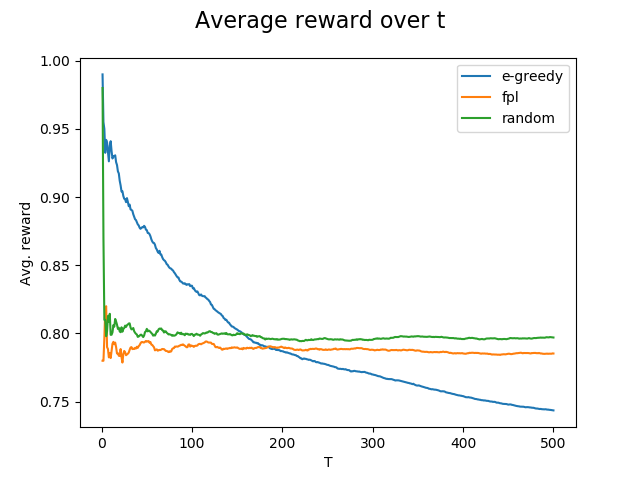
\includegraphics[width=0.9\textwidth]{img/Figure_1b.png}
\caption{The seeker's Exp3 strategy average reward}\label{fig1}
\end{figure}
\begin{figure}[!htb]
    \centering
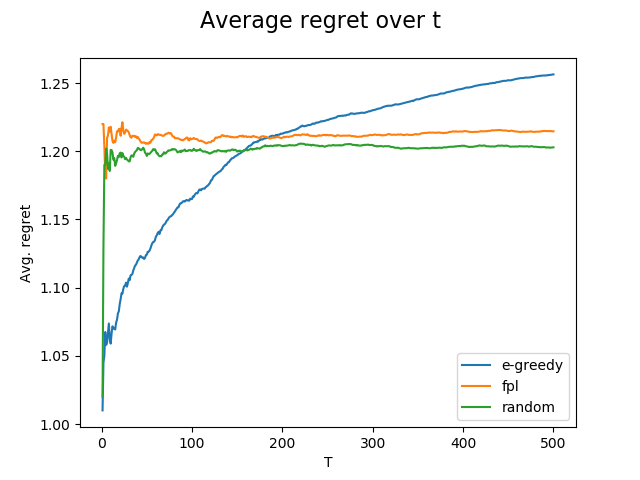
\includegraphics[width=0.9\textwidth]{img/Figure_2b.png}
\caption{The seeker's Exp3 strategy average regret}\label{fig2}
\end{figure}
\begin{figure}[!htb]
    \centering
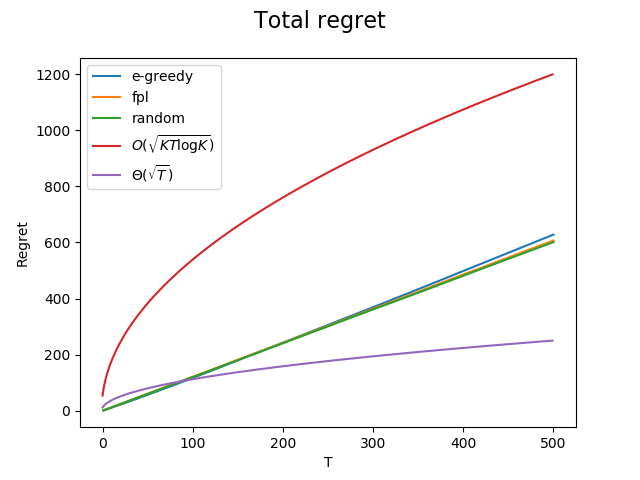
\includegraphics[width=0.9\textwidth]{img/Figure_3b.png}
\caption{The seeker's Exp3 strategy total regret}\label{fig3}
\end{figure}

As we can observe from figures \ref{fig1} and \ref{fig2} the hider's
strategies converge all to a uniform random strategy. In this type of
game, the uniform random strategy is the optimal strategy since it
cannot be learned and forces the opponent to play a uniform random
strategy as well. In this case, the epsilon-greedy and FPL strategies,
via a reward and frequency vector, keep track of their actions
consequences and update their values in order to minimize the
opponent's total reward. The seeker's Exp3 algorithm does something
similar by updating a weight vector, which describes the probability
of taking an action. In a 2 player capture the flag game setting with 2
flags and 5 sites the number of actions is described by all the
possible unique binary combinations of the sites. The resulting Exp3
strategy weights against uniform, epsilon-greedy and FPL strategies
result in a uniform (equiprobable) distribution. We can observe from
figure \ref{fig3} that Exp3 total expected regret is better than
$\sqrt{T}$, where $T$ is the number of timesteps, even when the
adversaries play optimal strategies (uniform random distribution in
this case).

All the implemented strategies, except the uniform random
one, face the exploration versus exploitation dilemma. At each
timestep the algorithms explore according to a small probability
degree. The algorithms, on the other hand, exploit by keeping track of
the previous interactions with the environment by using weight,
frequency or reward history vectors. We have to note that FPL
adaptivity strongly depends on the exponential distribution $\eta$
parameter. When using a fixed $\eta$ the exponential distribution at
the core of the algorithm does not affect the non-normalized action
weights anymore. An adaptive $\eta$ is needed in order to not fully
separate the exploration versus exploitation phases. The code
implementing the algorithms and plots of the results can be found in
appendix \ref{appendix}.


\begin{thebibliography}{8}

\bibitem{rlbook}
Sutton, R.S. and Barto, A.G., 2011. Reinforcement learning: An introduction.

\end{thebibliography}

\section{Appendix A: source code}\label{appendix}
This appendix section contains the source code of the implemented program.

\subsection{capture\_the\_flag.py}\label{capture_the_flag.py}
\lstinputlisting[language=Python]{../capture_the_flag.py}


\end{document}
